% Manuel Lippert - Paul Schwanitz
% Physikalisches Praktikum

% Auswertung Teil 1

\section{invertierteres Pendel}
\label{sec:auswertungPendel}
\subsection{Bifurkationsdiagramm und kritische Masse}
\label{sub:bifuAndKritMass}
Über den Versuch wurde die Auslenkung $\theta$ bzw. die Spannung $U_a$ am Digitalmultimeter links ($U_{a,l}$) und rechts ($U_{a,r}$) gemessen. Dabei ergeben sich erst ab einer gewissen Masse, eine Auslenkung links oder rechts hier schematisch in dem Bifurkationsdiagramm dargestellt (Abb \ref{image:bifu}), welches auch symmetrisch gegenüber Periode 1 ist.
\begin{center}
    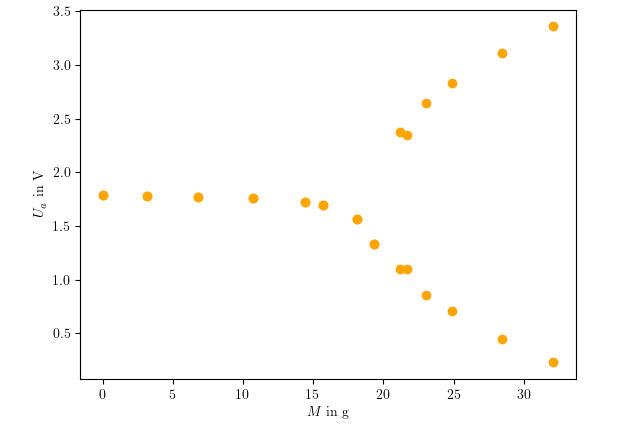
\includegraphics[scale=0.7]{Pendel/3.1/BifurkationMass.png}
    \captionof{figure}{Bifurkationsdiagramm in Abhängigkeit der Masse}
    \label{image:bifu}
\end{center}
Um die kritische Masse $M_k$ zu bestimmen, wird die Differenz $\Delta U_a=U_{a,l}-U_{a,r}$ bestimmt und diese quadriert, also $(\Delta U_a)^2$. Der Fehler ergibt sich dann aus dem Fehlerfortpflanzungsgesetz, wobei der Ablesefehler $s_a$ gleichzeitig als Restfehler $s_r$ abgeschätzt wird. Daraus folgt:
\begin{gather}
    (\Delta U_a)^2 = (U_{a,l}-U_{a,r})^2\\
    s_{U_a}=\sqrt{s_a^2+s_r^2}=\sqrt{2}s_a\\[0,5cm]
    s_{(\Delta U_a)^2}=\sqrt{\left(\frac{\partial((\Delta U_a)^2)}{\partial U_{a,l}}s_{U_a}\right)^2 + \left(\frac{\partial((\Delta U_a)^2)}{\partial U_{a,r}}s_{U_a}\right)^2}=2\sqrt{2}s_{U_a}|\Delta U_a|=4s_a |\Delta U_a|
\end{gather}
\begin{center}
    \begin{tabular}{r|cccc|cc}
        $M$/g &  $U_{a,l}$/V &  $U_{a,r}$/V & $s_a$/V & s_{U_a}/V & $(\Delta U_a)^2$/V$^2$ &  $s_{(\Delta U_a)^2}$/V$^2$ \\
        \hline
         0,00  &  1,78606 &  1,78606 &   0,00005 &  0,00007 &  0,0 &     0,0 \\
         3,14  &  1,78046 &  1,78046 &   0,00050 &  0,00071 &  0,0 &     0,0 \\
         6,78  &  1,77300 &  1,77300 &   0,00500 &  0,00707 &  0,0 &     0,0 \\
        10,75  &  1,76000 &  1,76000 &   0,00500 &  0,00707 &  0,0 &     0,0 \\
        14,42  &  1,72000 &  1,72000 &   0,05000 &  0,07071 &  0,0 &     0,0 \\
        15,72  &  1,70000 &  1,70000 &   0,05000 &  0,07071 &  0,0 &     0,0 \\
        18,10  &  1,57000 &  1,57000 &   0,05000 &  0,07071 &  0,0 &     0,0 \\
        19,36  &  1,33000 &  1,33000 &   0,05000 &  0,07071 &  0,0 &     0,0 \\
        21,19  &  1,10000 &  2,38000 &   0,05000 &  0,07071 &  1,6 &     0,3 \\
        21,67  &  1,10000 &  2,35000 &   0,05000 &  0,07071 &  1,6 &     0,3 \\
        23,05  &  0,86000 &  2,65000 &   0,05000 &  0,07071 &  3,2 &     0,4 \\
        24,88  &  0,71000 &  2,83000 &   0,05000 &  0,07071 &  4,5 &     0,4 \\
        28,45  &  0,45000 &  3,11000 &   0,05000 &  0,07071 &  7,1 &     0,5 \\
        32,12  &  0,23000 &  3,36000 &   0,05000 &  0,07071 &  9,8 &     0,6 \\
    \end{tabular}
    \captionof{table}{Messreihe Auslenkung Gleichgewichtslage}
    \label{tab:gleichgewichtslage}
\end{center}
Die Daten werden dann mit dem Numpy-Modul linear gefittet, dabei werden nur die letzten sieben Datensätze verwendet werden, da sich $(\Delta U_a)^2$ erst ab da Veränderung zeigt (siehe Abb. \ref{image:linFit}). Dabei ergibt sich die gefittete Funktion mit den jeweiligen Fehlern ermittelt:
\begin{gather}
    (\Delta U_a)^2 = c M + b = 0,77 \frac{\text{V}^2}{\text{g}} M - 14,73~\text{V}^2\\
    c = (0,77 \pm 0,02)~\frac{\text{V}^2}{\text{g}},~b = (-14,73 \pm 0,48)~\text{V}^2
\end{gather}
Daraus ergibt sich die kritische Masse $M_k$, wenn man $(\Delta U_a)^2=0$ setzt. Woraus widerrum mit Fehlerfortpflanzung folgt:
\begin{gather}
    M_k = \frac{b}{c} = 19,22~\text {g},~
    s_{M_k} = \sqrt{\left(\frac{s_b}{c}\right)^2+\left(\frac{b s_c}{c^2}\right)^2}=0,78~\text{g}\\[0,5cm]
    \Rightarrow\boxed{M_k = (19,22 \pm 0,78)~\text{g}}
\end{gather}
Die Federkonstante $k$ und dessen Fehler ergibt sich dann mit dem Fehler der Länge $L$ (gemessen mit Stahlmaßstab), wobei die Erdbeschleunigung fehlerfrei angenommen wird:
\begin{gather}
    L = 0,37~\text{m}\\
    s_L=\sqrt{s_a^2+s_r^2}=\sqrt{(5\cdot 10^{-4}~\text{m})^2+(5\cdot 10^{-5}~\text{m}+\cdot 10^{-4}*L)^2} = 0,0006~\text{m}\\
    M_k = \frac{k}{gL} \Leftrightarrow k = M_k g L = 0,069762834~\text{Nm}\\
    s_k = \sqrt{(gLs_{M_k})^2+(M_kgs_L)^2} = 0,002833425~\text{Nm}\\[0,5cm]
    \Rightarrow\boxed{k = (0,070 \pm 0,003)~\text{Nm}}
\end{gather}
Hierbei ist anzumerken, dass $k$ nicht die Einheit einer Federkonstante hat sondern eines Drehmoments. Die Vermutung liegt mit einen Blick auf Kapitel \ref{sub:bewegungsgleichung} beschrieben Differentialgleichung, dass sich bei $k$ eigentlich um das Direktionsmoment handeln muss, wobei das Direktionsmoment der Federkonstante $k$ bei longitudinalen Auslenkungen entspricht.

Zur Verifikation des Ergebnisses haben wir mehrfache (10mal) die Schwingungsdauer des Pendels mit der befestigten Masse $M = 12,58$ g gemessen.
\begin{center}
    \begin{tabular}{ c | cccccccccc }
        {} & 1 & 2 & 3 &4 &5 &6 &7 &8 &9 &10\\
        \hline
        $T_10$/s&19,14&19,28&18,88&19,18&19,00&18,66&19,12&19,01&19,20&19,29\\
    \end{tabular}
    \captionof{table}{Messreihe Schwingungsdauer}
    \label{tab:schwingung}
\end{center}
Es wird nun der Mittelwert über eine Periode genommen, wobei der Ablesefehler der digitale Messuhr auch gleichzeitig als Restfehler abgeschätzt wird und der Fehler der einen Periode mit dem Fehlerfortpflanzungsgesetz berechnet wurde. Daraus folgt:
\begin{gather}
    T = \overline{T} = \frac{1}{10} \sum_{n = 1}^{10} \frac{T_{10,n}}{10} = 1,9076~\text{s}\\
    s_{T_{10}} = \sqrt{s_a^2+s_r^2}=\sqrt{2}s_a \Rightarrow s_T = \frac{s_T}{10\sqrt{10}} = \frac{s_a}{10\sqrt{5}} = 0,000447214\\[0,5cm]
    \Rightarrow\boxed{T = (1,9076 \pm 0,0004)~\text{s}}
\end{gather}
\newpage
Über Federkonstante (Direktionsmoment) $k$ lässt sich dann die Schwingungsdauer $T$ wie folgt berechnen \citep{Leifi}, wobei für den Fehler von $T$ der Fehler der Masse und Länge vernachlässigt wird:
\begin{gather}
    T = 2\pi\sqrt{\frac{ML^2}{k- MgL}} = 1,671383586~\text{s}\\
    s_T = \frac{\pi ML^2 s_k}{(k-MgL)^2 \sqrt{\frac{ML^2}{k- MgL}}} = 0,1030091566\\[0,5cm]
    \Rightarrow\boxed{T = (1,67 \pm 0,10)~\text{s}}
\end{gather}
Das Ergebnis zeigt, dass die bestimmte Federkonstante $k$ nahe an den tatsächlichen Wert der Blattfeder liegt. Die möglichen Abweichung könnten von denen in Kapitel \ref{sub:bewegungsgleichung} gemachten Näherungen oder dem vorangegangenen Fit verursacht werden. Auch könnte das Alter des Messaufbaus seinen Teil zu der Ungenauigkeit beigetragen haben. Dennoch ist das Ergebnis im Rahmen unserer Möglichkeiten akzeptabel.
\newpage
\begin{center}
    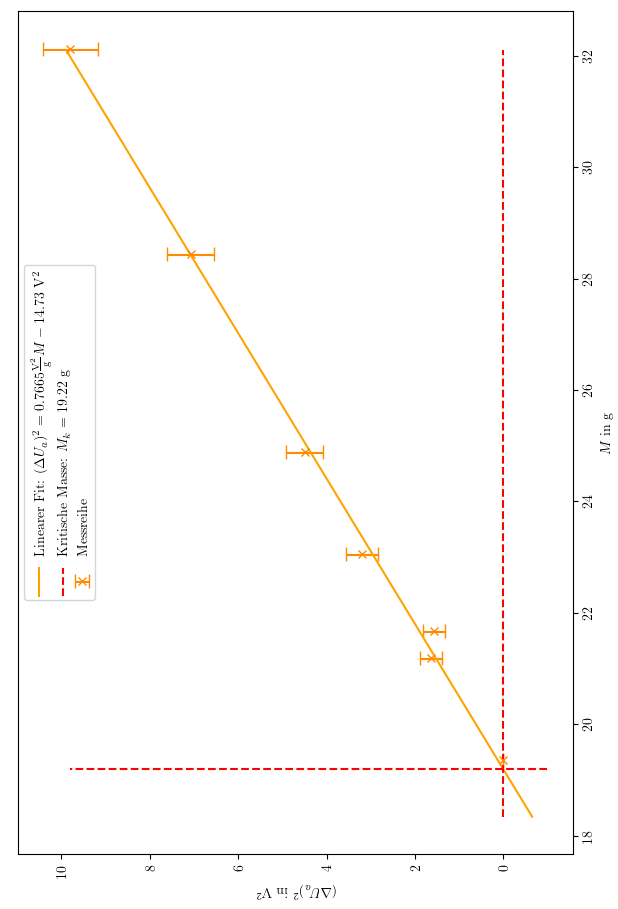
\includegraphics[scale=0.6]{Pendel/3.1/linearFit.png}
    \captionof{figure}{Linerar Fit der Messreihe}
    \label{image:linFit}
\end{center}
\subsection{Schwache Nichtlinearität}
\label{sub:AuswertungweakLin}
\paragraph{a)}
Für die experimentelle Auswertung der Amplitudenabhängigkeit der Schwingungsdauer $T$ des Pendels  wird aus den aufgenommenen Daten die Maxima von der Spannung $U_{a}$ bestimmt, sowie der zeitlichen Abstand $\Delta t$ zwischen zwei Maxima ermittelt. Bei den Abstand $\Delta t$ entspricht dann der Periodendauer $T$ des Pendels. Da mehrere Werte für $T$ verhäuft vorkamen, haben wir die Daten von $T$ gruppiert und über die zugehörigen Maxima der Spannung $U_{a,max}$ den Mittelwert gebildet.
\begin{center}
    \begin{tabular}{c|c}
        $T$/s & $U_{a,max}$/V\\
        \hline
        1.90  &  2.395000 \\
        2.10  &  2.231000 \\
        2.20  &  2.045000 \\
        2.30  &  1.881600 \\
        2.32  &  1.723000 \\
        2.36  &  1.540000 \\
        2.40  &  1.627824 \\
        2.44  &  1.565100 \\
        \end{tabular}
        \captionof{table}{Messreihe Schwingungsdauer in Amplitudenabhängigkeit}
\end{center}
\begin{center}
    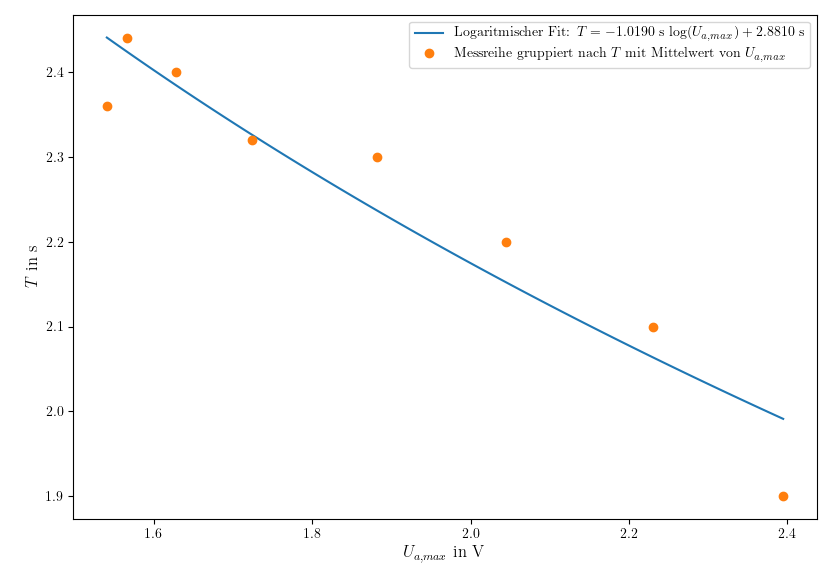
\includegraphics[scale=0.5]{Pendel/3.2a/AbhSchwingung.png}
    \captionof{figure}{Ampliudenabhängigkeit der Schwingungsdauer mit logarithmischen Fit}
    \label{image:schwing}
\end{center}
Bei der grafischen Auswertung (siehe Abb.\ref{image:schwing}) erkennt man deutlich einen Abwärtstrend. Ein logarithmischer Fit wie in Kapitel \ref{sub:schwingungsdauer} beschrieben, gibt dann die Funktion:
\begin{gather}
    T=(-1,0190~\text{s})\log(U_{a,max}) + (2.8810~\text{s}).
\end{gather}
Dieser Fit ist aber noch nicht Aussagekräftig, da die Messwerte auch einen linearen Fir zulassen würden, weswegen mehr Messpunkte gebraucht werden würden.
\paragraph{b)}
\begin{center}
    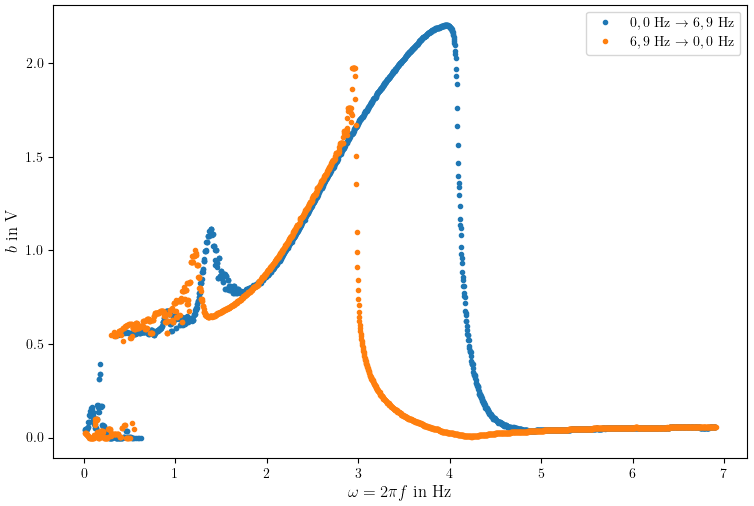
\includegraphics[scale=0.7]{Pendel/3.2b/Resonanz.png}
    \captionof{figure}{Resonanzkurve}
    \label{image:resonanz}
\end{center}
Bei der Messung der Resonanzkurve erkennt man grob verschiedene Bereiche, dabei beschreibt die Aufwärtsbewegung die blaue Kurve (0,0 Hz $\rightarrow$ 6,9 Hz) und die Abwärtsbewegung die orange Kurve (6,9 Hz $\rightarrow$ 0,0 Hz):
\begin{itemize}
    \item[1)]0,0-0,5 Hz\\Die Drehfrequenz des Schrittmotors reicht nicht aus um das Pendel anzuregegen.
    \item[2)]0,5-2,0 Hz\\Erregerfrequenz regt Pendel zum schwingen an. Vereinzelte Zacken zeigen dabei die Schritte, welche der Schrittmotor macht beim Antreiben.
    \item[3)]2,0-3,0 Hz\\Anstieg der Amplitude und Fall Abwärtsbewegung erreicht die Kurve ihr Maximum.
    \item[4)]3,0-4,0 Hz\\Anstieg der AUfwärtsbewegung zu ihrem Maximum, während die Abwärtsbewegung in den instabilen Zustand (siehe Abb. \ref{image:resonanzkurve}) übergeht.
    \item[5)]4,0-5,0 Hz\\Abfallen der Aufwärtsbewegung und übergehen der Aufwärtsbewegung in die Abwärtsbewegung.
    \item[6)]5,0-6,9 Hz\\Pendel kommt Drehfrequenz des Motors nicht mehr hinterher und schwingt nicht mehr 
\end{itemize}
\subsection{Starke Nichtlinearität}
\label{sub:AuswertungstrongLin}
\paragraph{a)}
Nun werden die einzelnen Schwingungszustände bei verschiedenen Frequenzen untersucht. Wobei mit einer hohen Frequenz begonnen wurde und dann schrittweise verkleinert wird. Dabei ist durch den Ausfahl des Messprogramms zwei Messreihen erstellt, wodurch sich der Attraktoren verändert hat. 
\begin{center}
    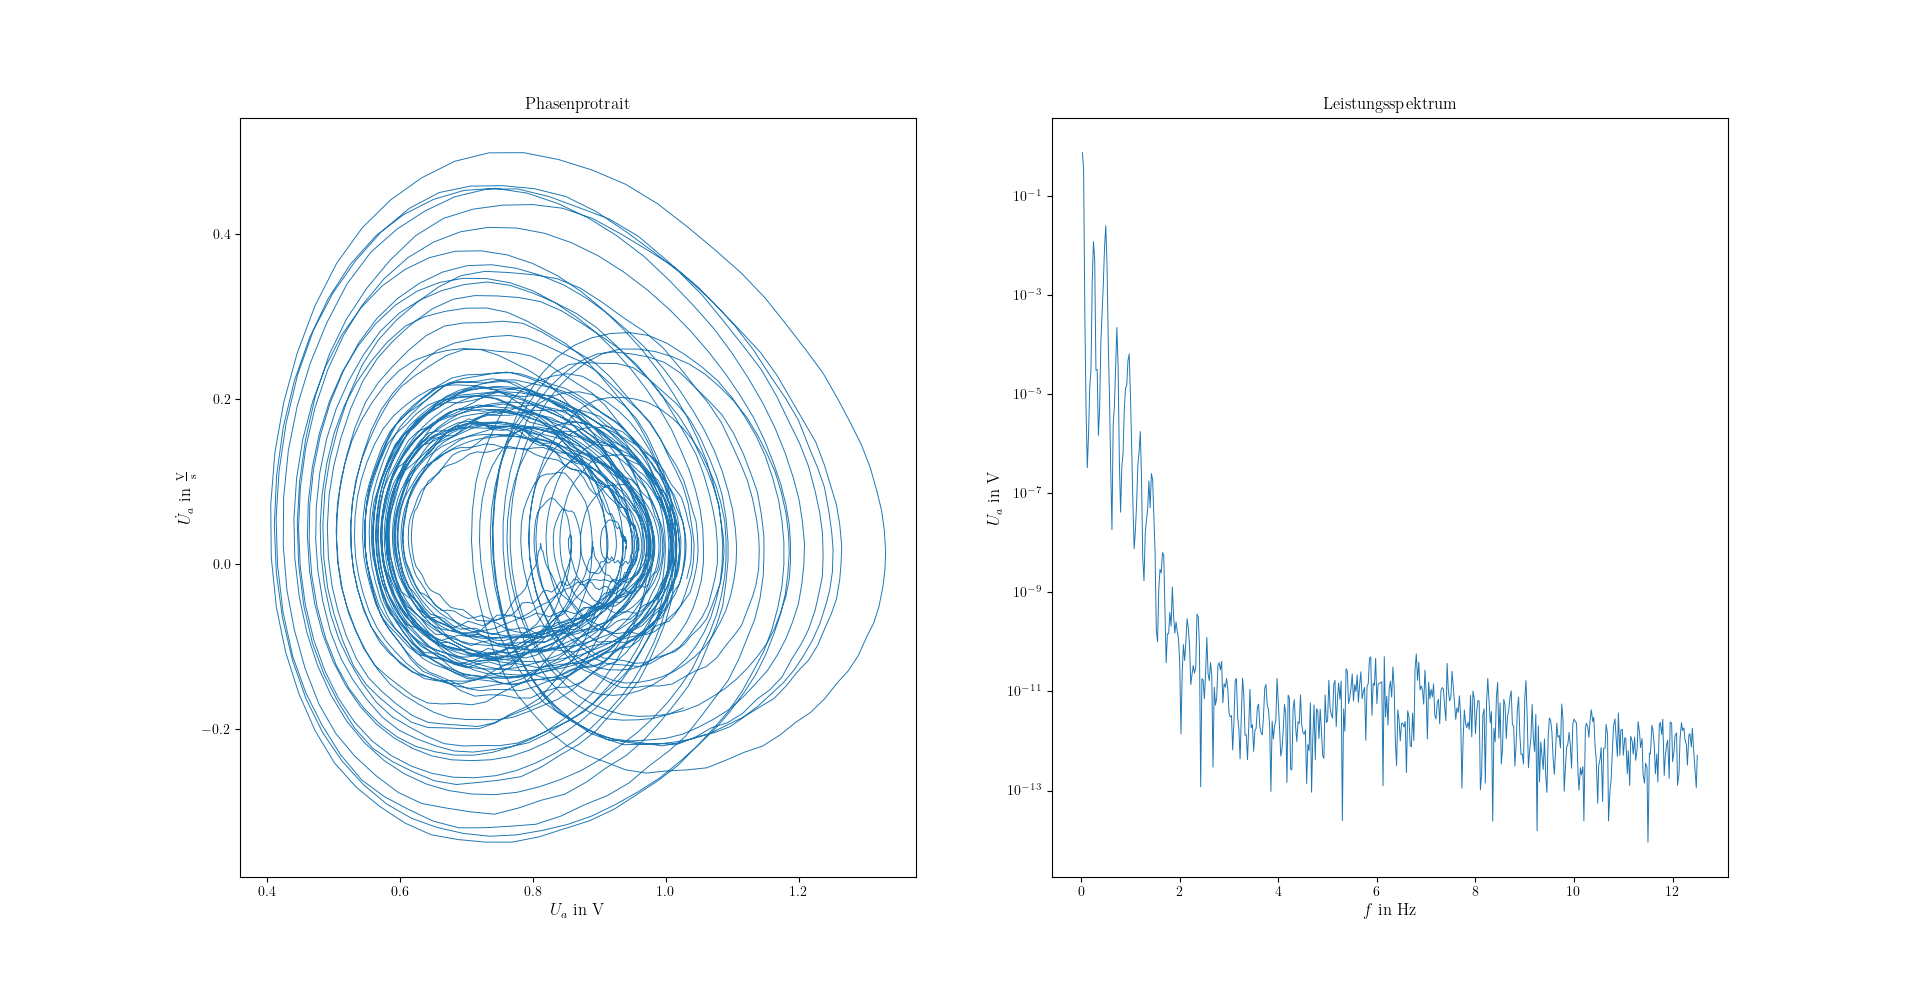
\includegraphics[scale=0.3]{Pendel/3.3a/0,233Hz.png}
    \captionof{figure}{0,233 Hz}
    \label{image:0,233hz}
    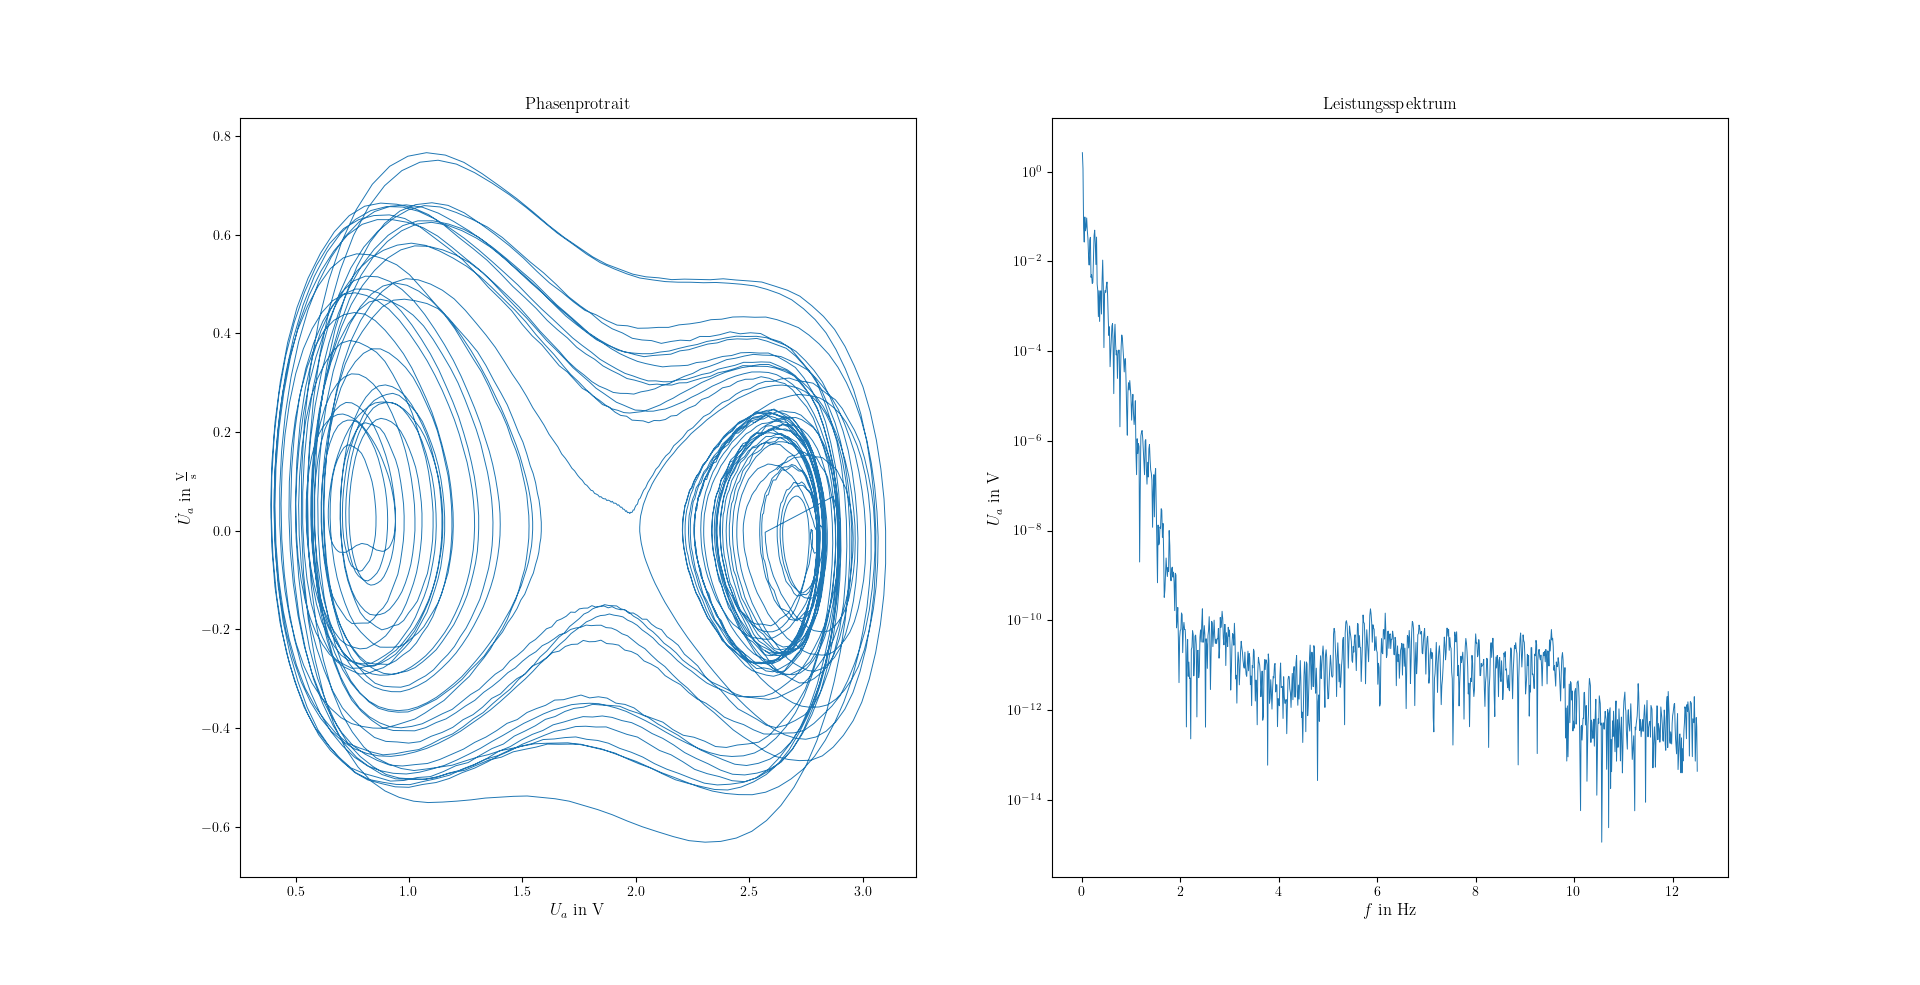
\includegraphics[scale=0.3]{Pendel/3.3a/0,411Hz.png}
    \captionof{figure}{0,411 Hz}
\end{center}
Chaotisches Verhalten, was in Leistungsspektrum auch zu erkennen ist. Weiterhin erkennt man die zwei möglichen Schwingungen auf der rechten und linken Seite der Pendels. In der Mitte ist dabei ein Sattelpunkt des Attraktors. Die Abb. \ref{image:0,233hz} beschreibt dabei die Schwingung auf der linken Seite.
\begin{center}
    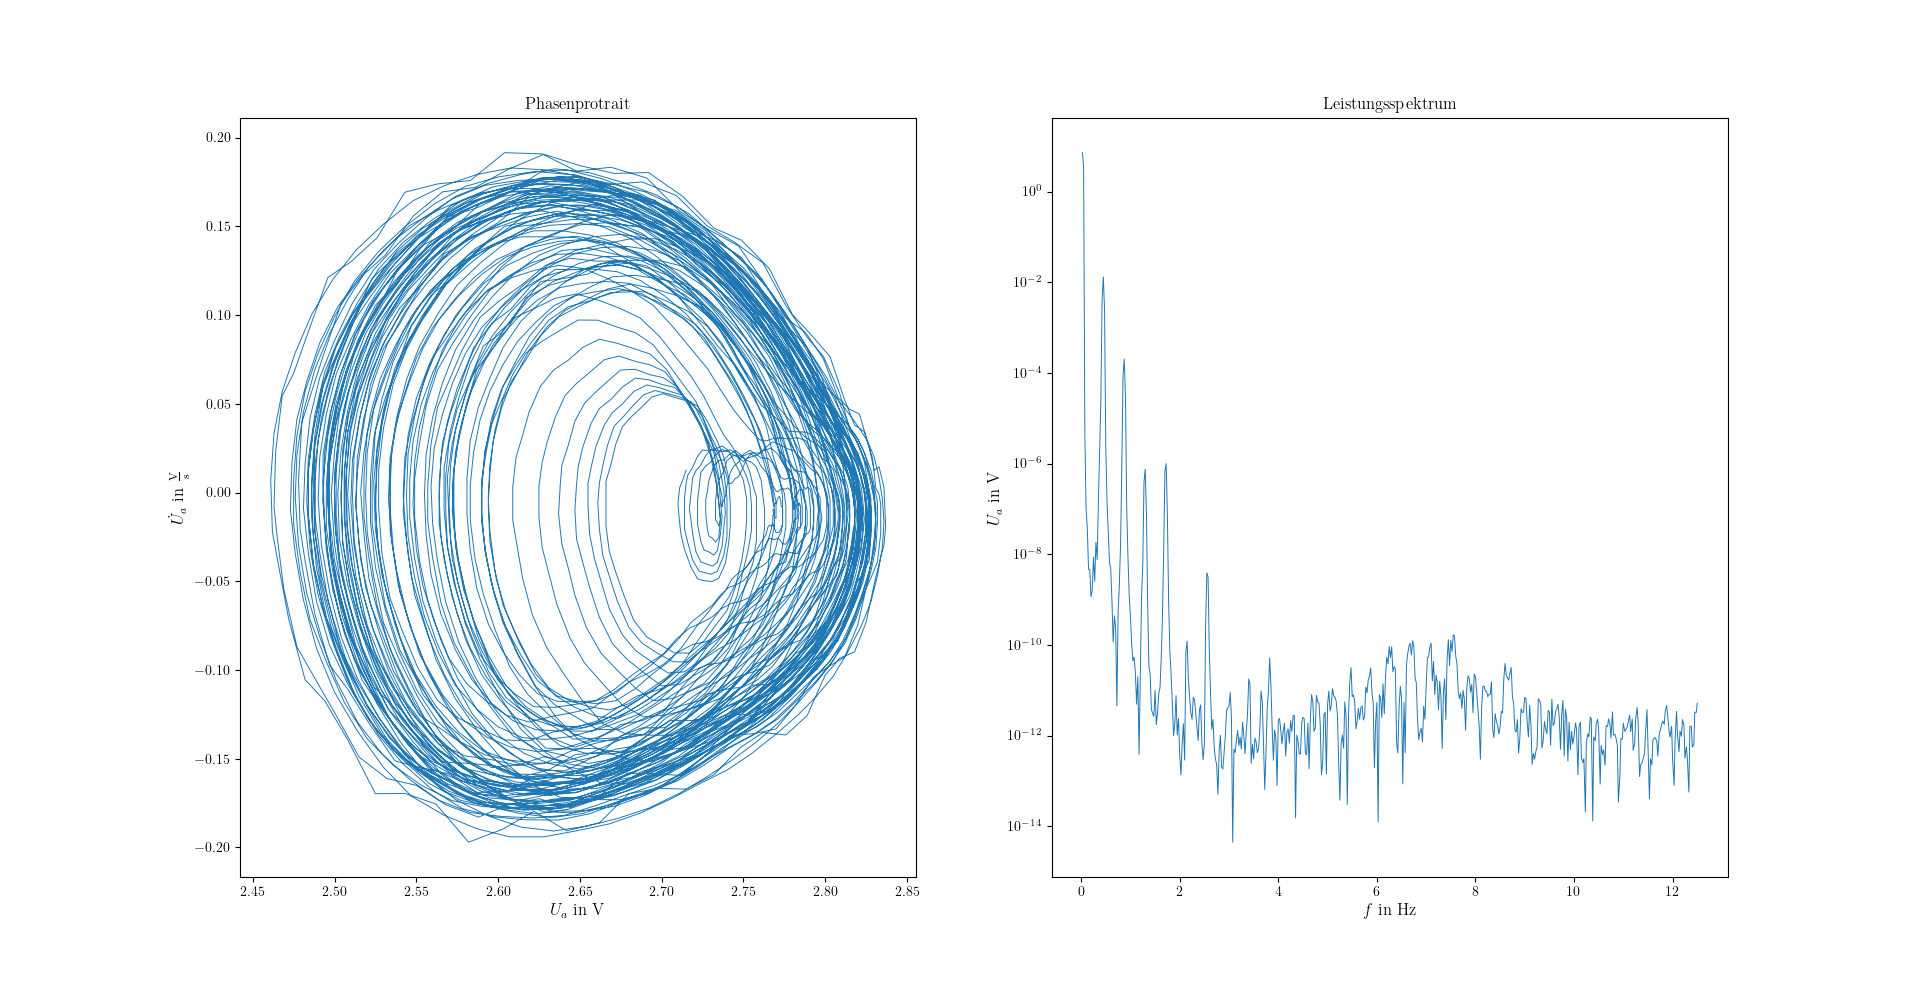
\includegraphics[scale=0.3]{Pendel/3.3a/0,847Hz.png}
    \captionof{figure}{0,847 Hz}
    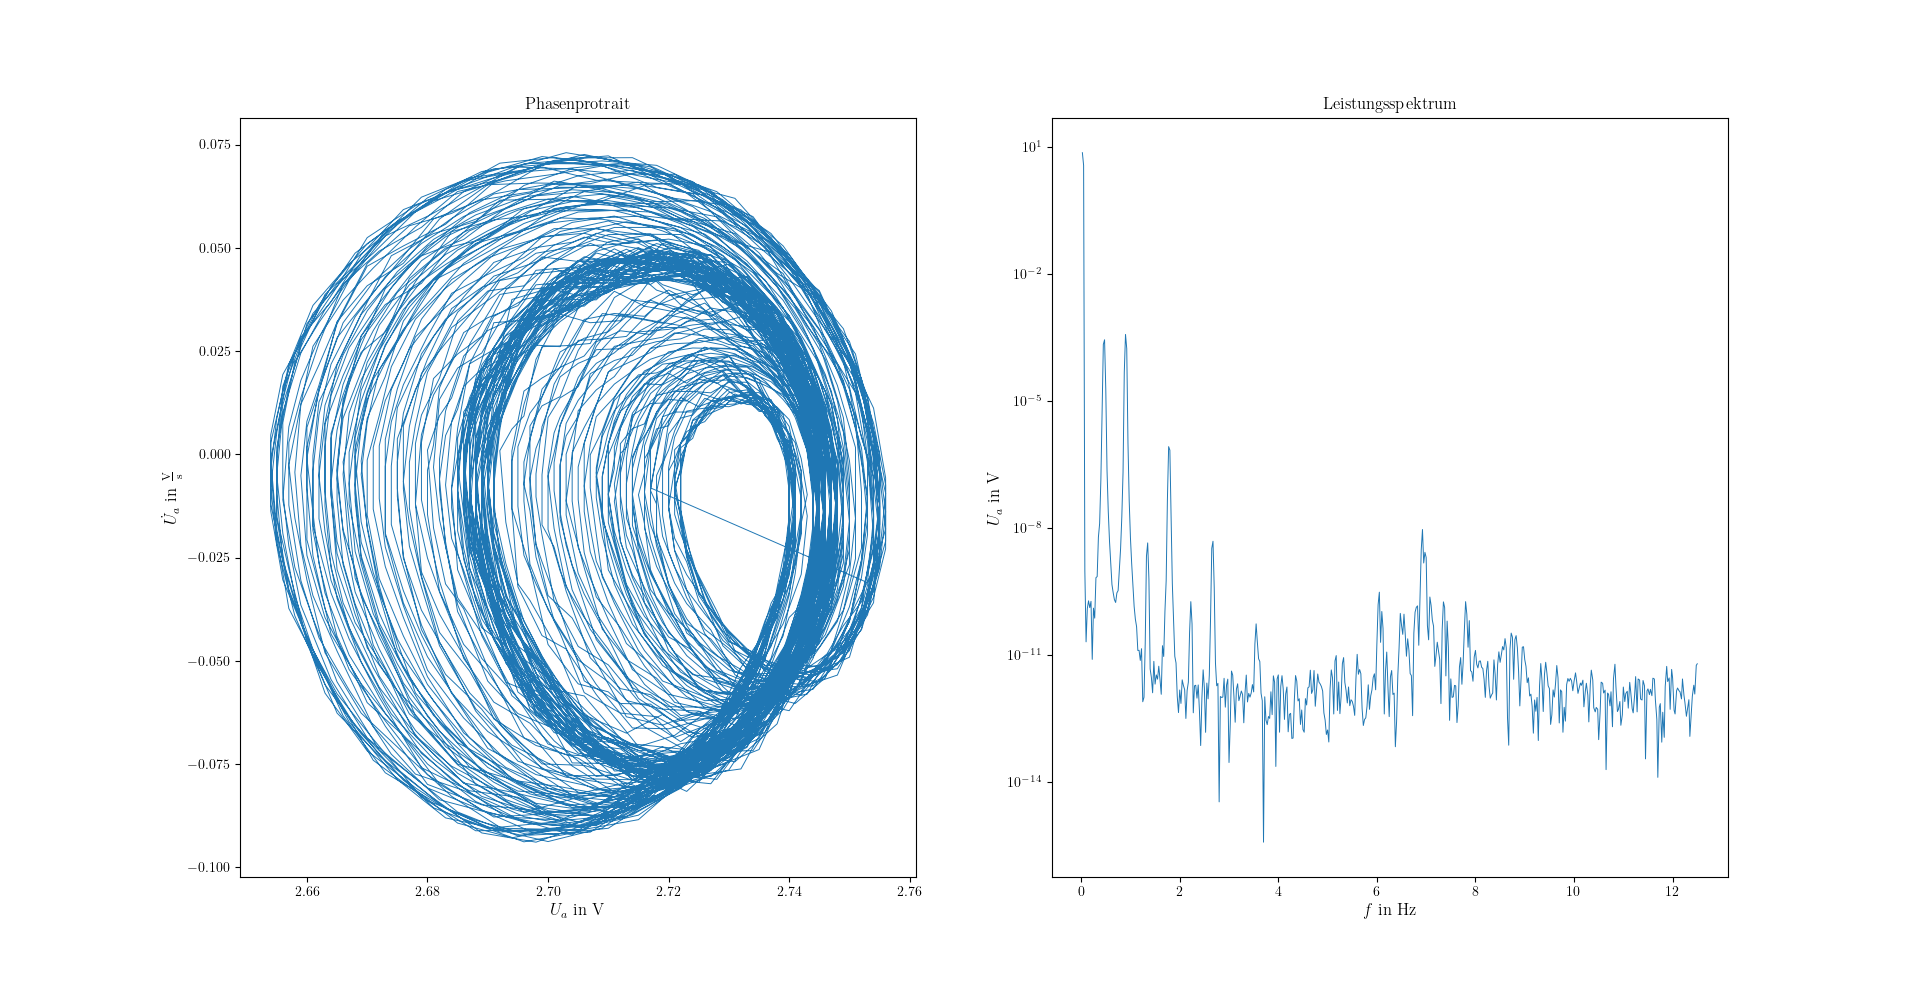
\includegraphics[scale=0.3]{Pendel/3.3a/0,882Hz.png}
    \captionof{figure}{0,882 Hz}
\end{center}
Hier erkennt man schon die Periode 2 in leichter Ausprägung, dennoch ist das Verhalten weiter chaotisch, wobei im Leistungsspektrum mehrere deutliche Peaks zu erkennen sind.
\begin{center}
    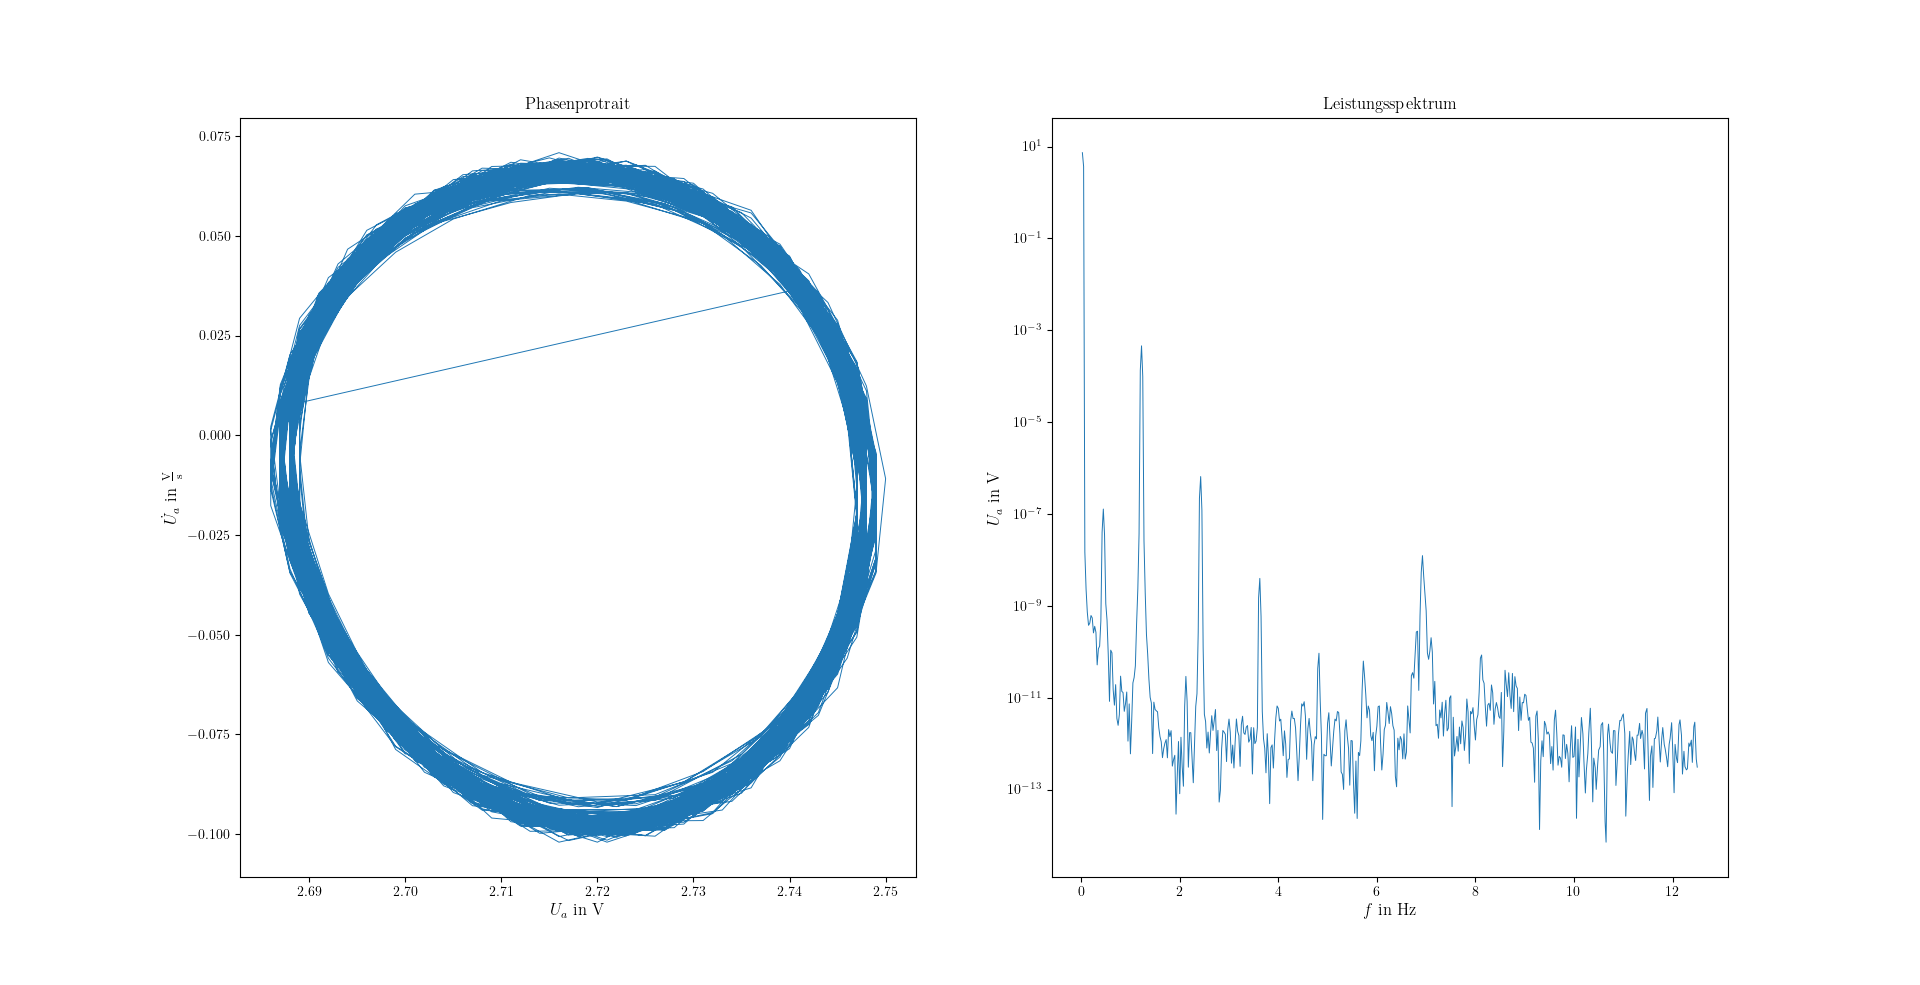
\includegraphics[scale=0.3]{Pendel/3.3a/1,201Hz.png}
    \captionof{figure}{1,201 Hz}
\end{center}
Deutliches Ausbilden der Periode 1 gut zu erkennen an den definierten Peaks im Leistungsspektrum.
\begin{center}
    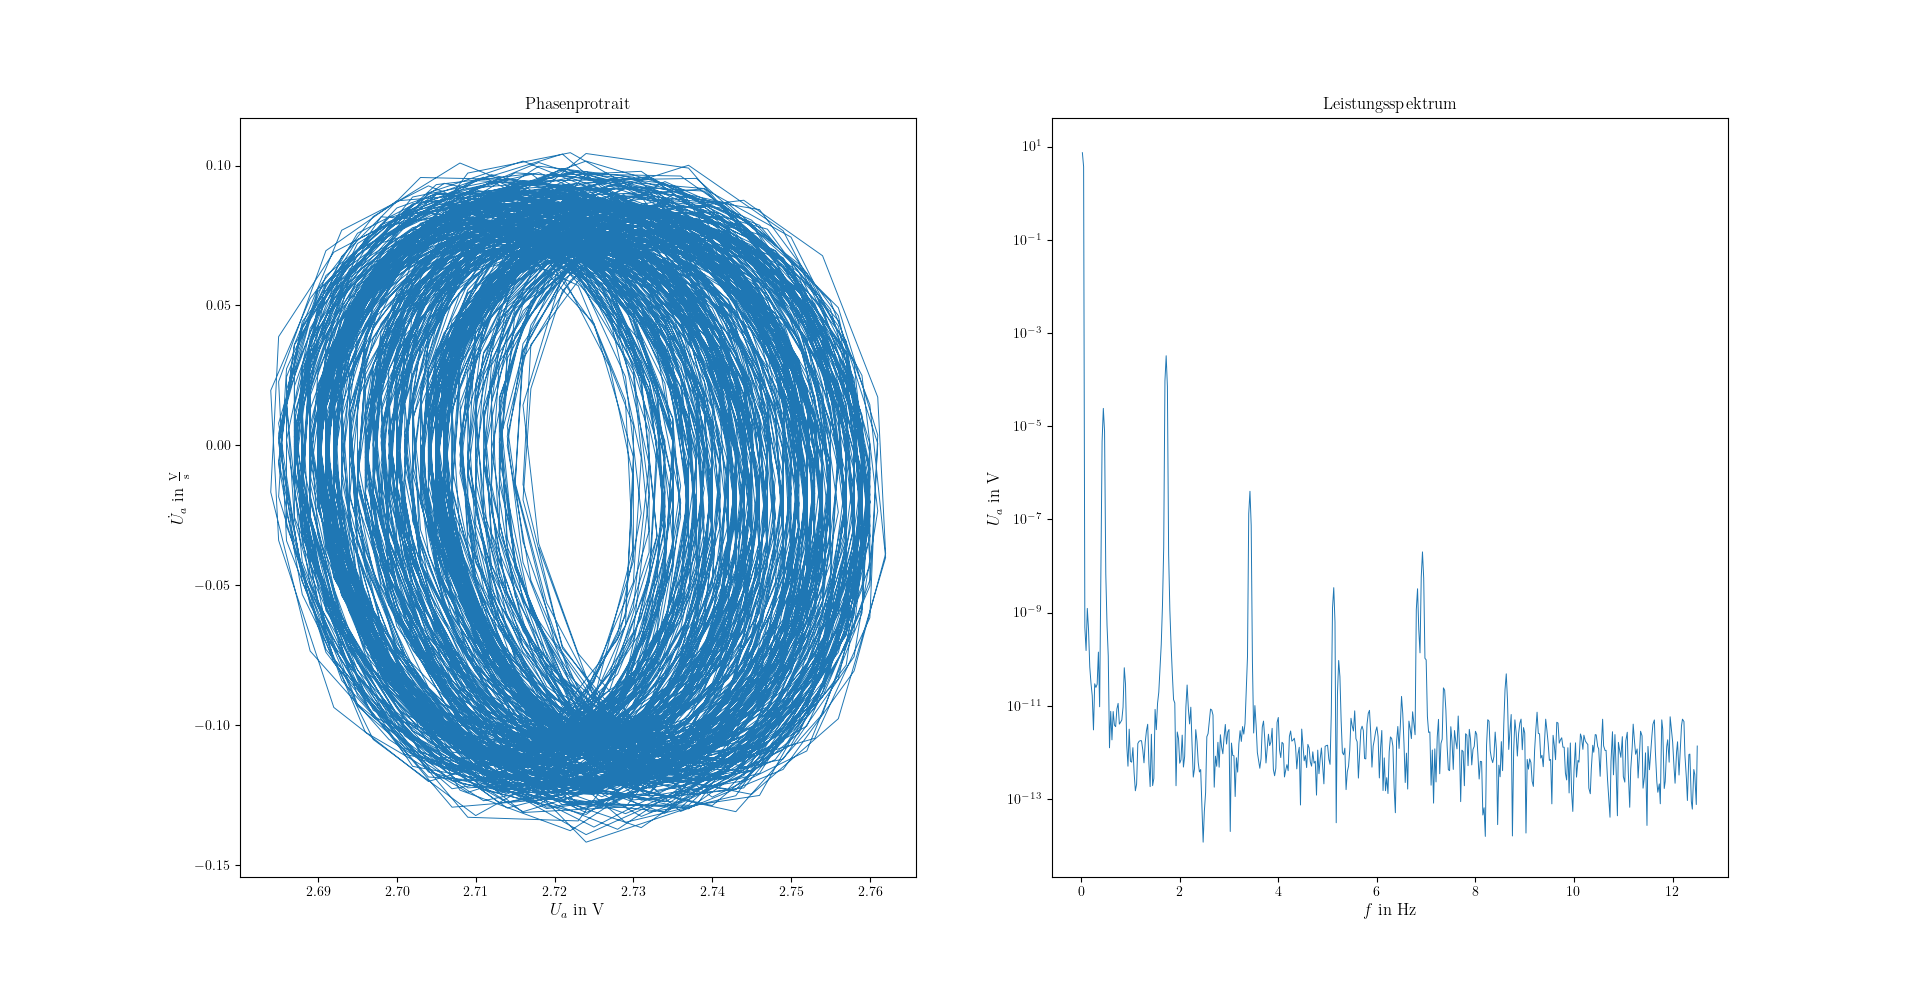
\includegraphics[scale=0.3]{Pendel/3.3a/1,702Hz.png}
    \captionof{figure}{1,702 Hz}
    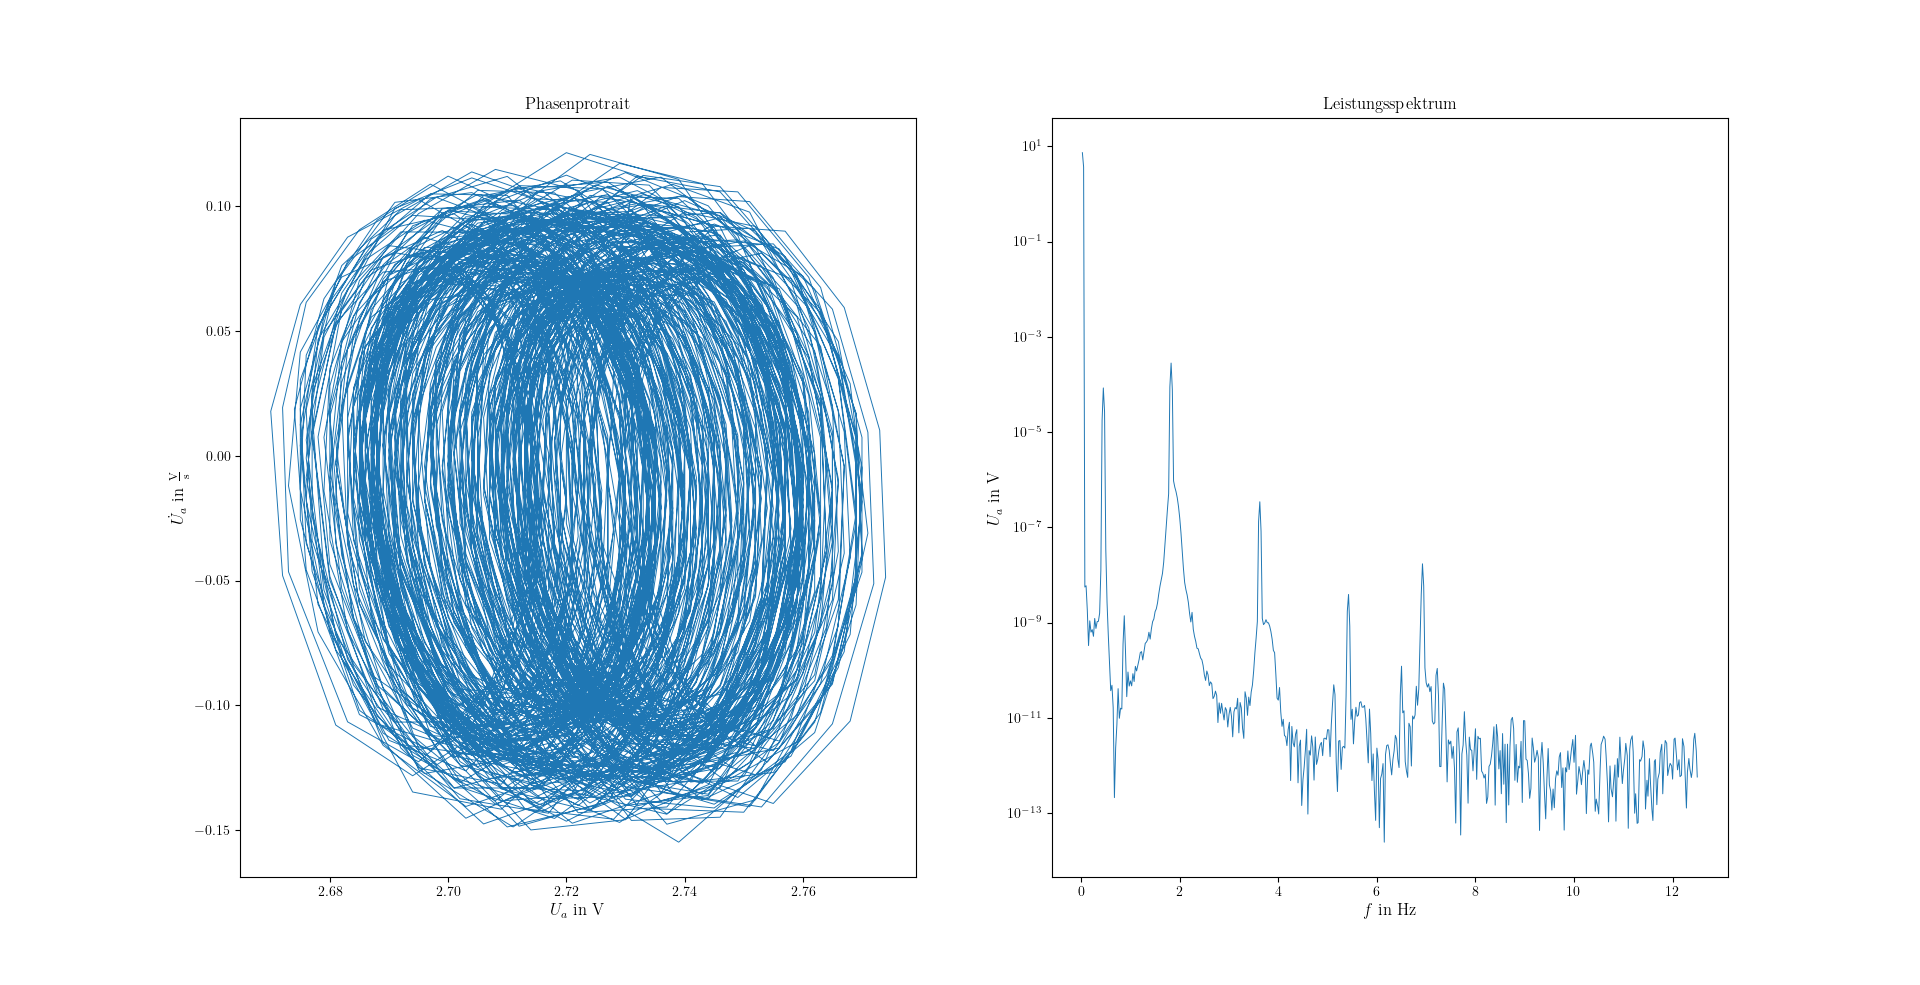
\includegraphics[scale=0.3]{Pendel/3.3a/1,802Hz.png}
    \captionof{figure}{1,802 Hz}
    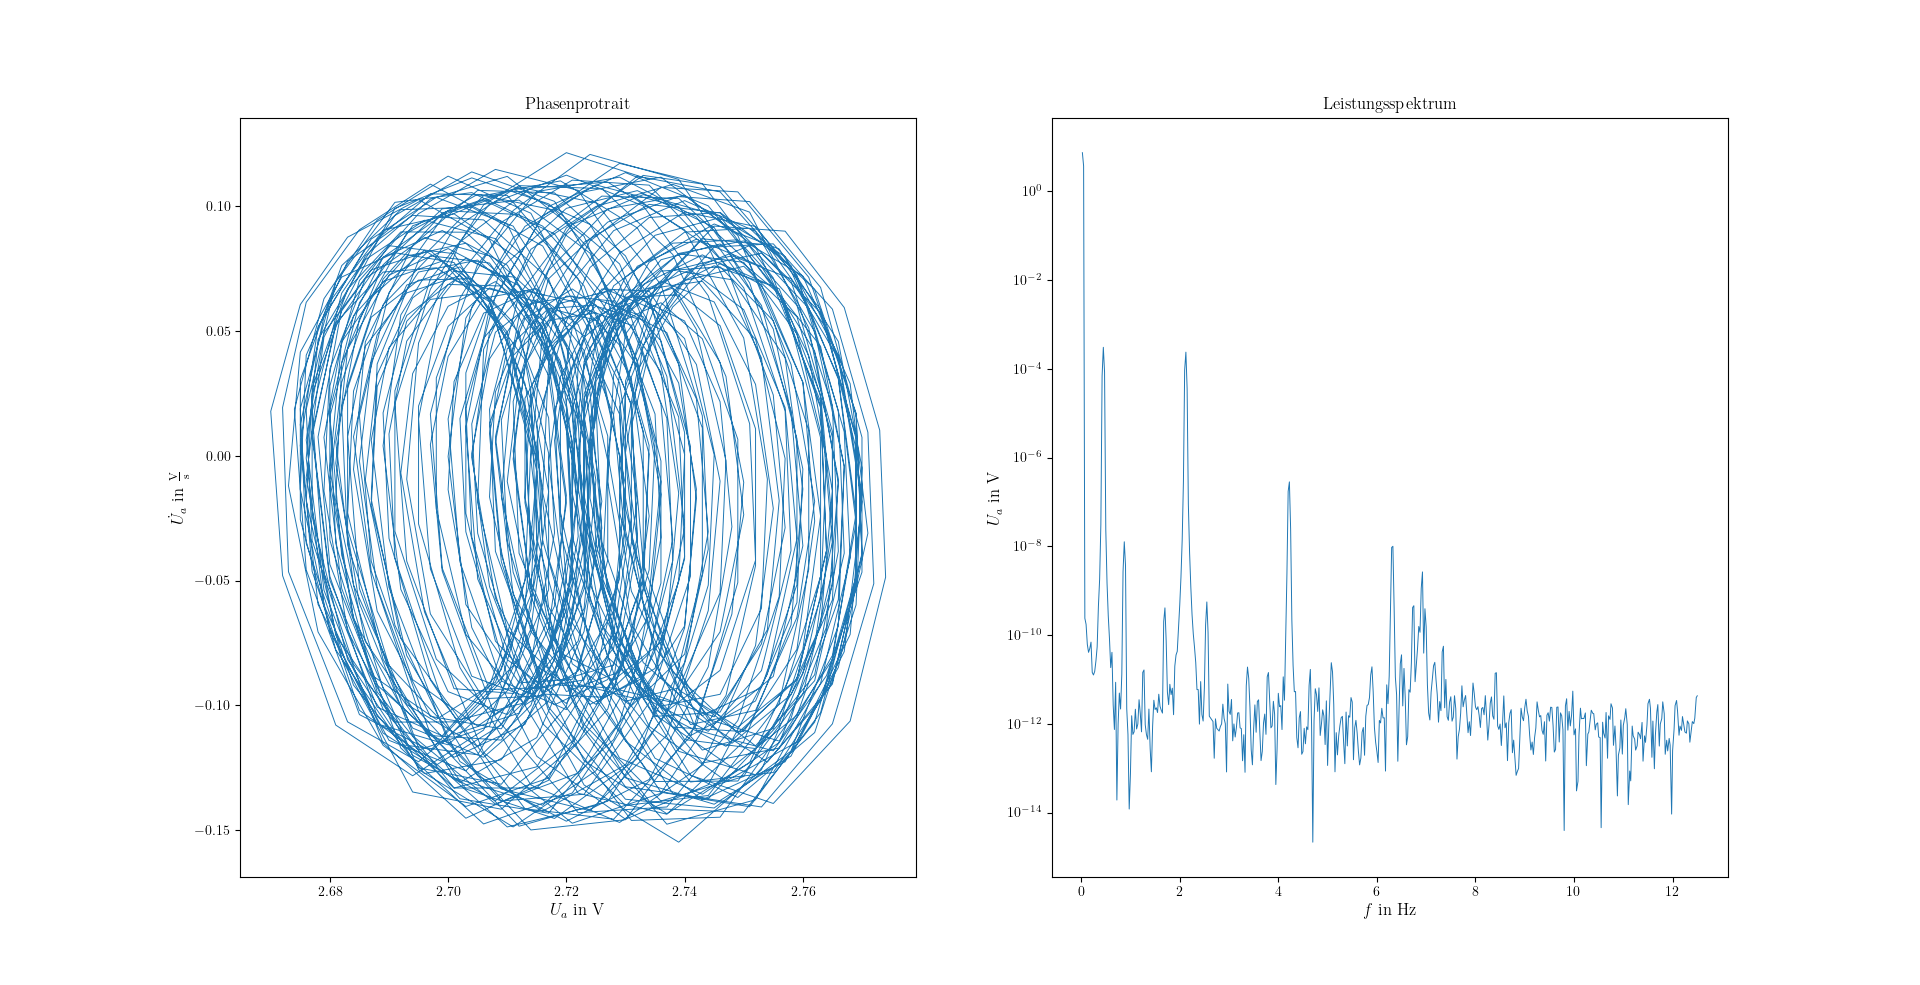
\includegraphics[scale=0.3]{Pendel/3.3a/2,100Hz.png}
    \captionof{figure}{2,100 Hz}
\end{center}
Ausprägen des Torusattraktors bei höheren Frequenzen, wobei dabei das Leistungsspektrum unverändert an der Anzahl der Peaks bleibt, aber die Ausprägung ändert sich.
\newpage
\paragraph{b)}
\begin{center}
    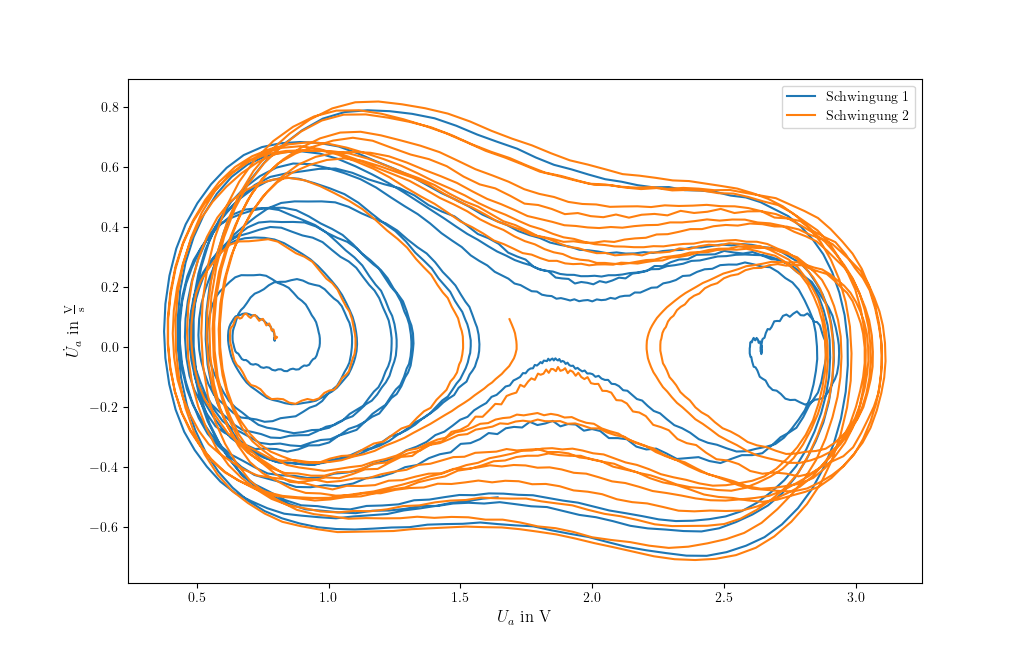
\includegraphics[scale=0.5]{Pendel/3.3b/Schwingungall.png}
    \captionof{figure}{Schwingung kompletten Datensatz dargestellt}
    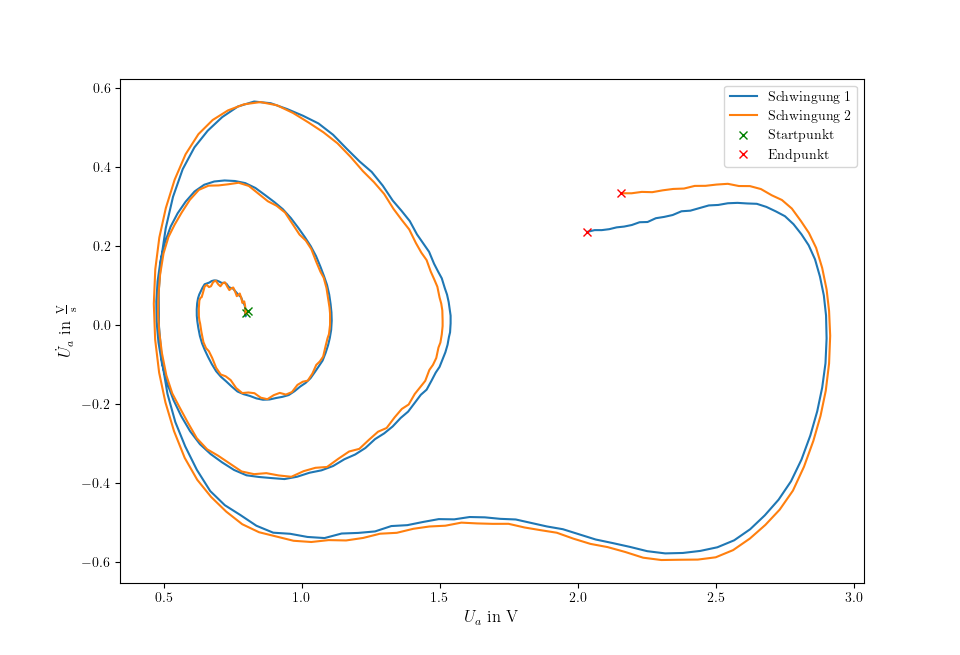
\includegraphics[scale=0.5]{Pendel/3.3b/Startwert.png}
    \captionof{figure}{Schwingung mit Start und Endpunkt}
    \label{image:startwert}
\end{center}
In Abbildung \ref{image:startwert} erkennt man dann deutlich, dass die Schwingungen sich beim zweiten Umschlag auf die linken Seite voneinander unterscheiden. 